\begin{comment}

Keywords:

    - [x, y, t, p, a, l]
    - JSON -> Dataframe
    - [x, y, t, p, a, l, stroke number]
    - Pandas Dataframe, effectively store and analyze 
    - Dataframe + Metadata = Drawing Entity
    - Outliers removal 
    
        In statistics, an outlier is an observation point that is distant from other observations. An outlier may be due to variability in the measurement or it may indicate experimental error; the latter are sometimes excluded from the data set.
        
        Our approach was to remove the outlier points by eliminating any points that were above (Mean + 2*SD) and any points below (Mean - 2*SD) before plotting the frequencies
        
        For a random variable vector A made up of N scalar observations, the median absolute deviation (MAD) is defined as

        MAD = median(A
        i
        −median(A))
        for i = 1,2,...,N.
        
        
        For example, isoutlier(A,'mean') returns true for all elements more than three standard deviations from the mean.
        

\end{comment}

\section{Data description}

On initial stage of algorithm, we process list of JSON transport objects, which represents separate drawings. Each JSON file has specific name and collection of fields, filled with meta-information about corresponding drawing, such as \textit{[patientId, session, time, type]} and drawing data, which is list of strokes, stroke is a list of points and point is aforementioned vector of \textit{[x, y, t, p, a, l]}. Sample JSON file is shown in the following listing.

\begin{table}[htb]
\centering
\begin{lstlisting}

{ "session": "2CEE8303-8AD9-4D42-AFCA-0966DAA3E7FE",
  "type": "plcopy",
  "time": "2018-03-05 06:48:43 +0000",
  "patientId": "PD-15"
  "data": [
    [ { "x": 41.5938, "l": 0.96508, "a": 1.03885,
        "y": 213.914, "p": 0.33333, "t": 541925323.7092 },
      { "x": 52.4063, "l": 0.91419, "a": 2.18995,
        "y": 215.097, "p": 0.00001, "t": 541925324.55801 } ...] ...
  ]}

\end{lstlisting}
\caption{Listing --- Sample JSON drawing file}
\end{table}

\section{Drawing Entity}

% Pandas dataframe is two-dimensional matrix with labeled columns and rows. Columns can potentially store different types of data. We can think of dataframe as a spreadsheet or SQL table.

% Two-dimensional size-mutable, potentially heterogeneous tabular data structure with labeled axes (rows and columns). Arithmetic operations align on both row and column labels. Can be thought of as a dict-like container for Series objects. The primary pandas data structure

To effectively store and manipulate the data, we introduced Drawing Entity, which essentially is a wrapper object around existing JSON file with populated meta-information and drawing data transformed into single Pandas dataframe. 

\begin{table}[htb]
\centering
\begin{tabular}{@{}c|c|c@{}}
\hline
Field       & Description                         & Type     \\
\hline
name        & Original name of the JSON file      & String   \\
testType    & Type of the drawing test            & String   \\
patientType & Class of tested individual          & String   \\
dateTime    & Timestamp when drawing was recorded & DateTime \\
\hline
\end{tabular}
\caption{Drawing Entity --- Metadata}
\label{metadata}
\end{table}

Pandas dataframe is two-dimensional matrix with labeled columns and rows. Columns can potentially store different types of data. We can think of dataframe as SQL table or spreadsheet. On current stage of algorithm whole list of JSON files transformed into Drawing objects. Small transformation was necessary to perform: drawing JSON data
was represented as list stroke, and stroke is a of list of points. Multiple array analysis seemed not much flexible and we flattened whole structure into single dataframe of points and populated additional column with $i$ variable, representing stroke index of current point. Final dataframe structure and Drawing entity meta-information are described on Tables \ref{dataframe} and \ref{metadata}

% (Table \ref{dataframe} on page \pageref{dataframe})

\begin{table}[htb]
\centering
\begin{tabular}{c|c|c|c}
\hline
Feature & Description    & Unit                                & Type    \\
\hline
x       & x - coordinate & mm                                  & Float   \\
y       & y - coordinate & mm                                  & Float   \\
t       & time stamp     & sec                                  & Float   \\
p       & vertical pressure       & abstract unit, range {[}0..6.0{]} & Float   \\
a       & altitude angle & degrees                             & Float   \\
l       & latitude angle & degrees                             & Float   \\
i       & stroke index   & number                              & Integer \\
\hline
\end{tabular}
\caption{Drawing Entity --- Dataframe Structure}
\label{dataframe}
\end{table}

\subsection{Outlier removal}

An \textit{outlier} is a separate observation, which is located relatively far from other observations. During intermediate process of \textit{JSON} transport object conversion into \textit{Drawing} entity, we apply \textit{outlier} removal function to the \textit{dataframe}. 

To determine outliers, we use simple heuristics, that all Luria patterns tend to have horizontal direction and always limited in vertical range, therefore we should not have significant deviation by $y$-coordinate. We treat arbitrary data point $p_i$ in vector of points $[p_1, p_2 ..., p_{n-1}, p_n]$ as an outlier, if scalar value $y_i$ of vector of all y-coordinates $[y_1, y_2, ...y_{n-1}, y_n]$ is more than three standard deviations away from the vector $[y_1, y_2, ...y_{n-1}, y_n]$ average.

\subsection{JSON to Drawing entity Conversion}

Final transformation process of JSON transport object to \textit{Drawing} entity is exposed on Figure \ref{alg-drawing}

\begin{figure}[htb]
  \centering
    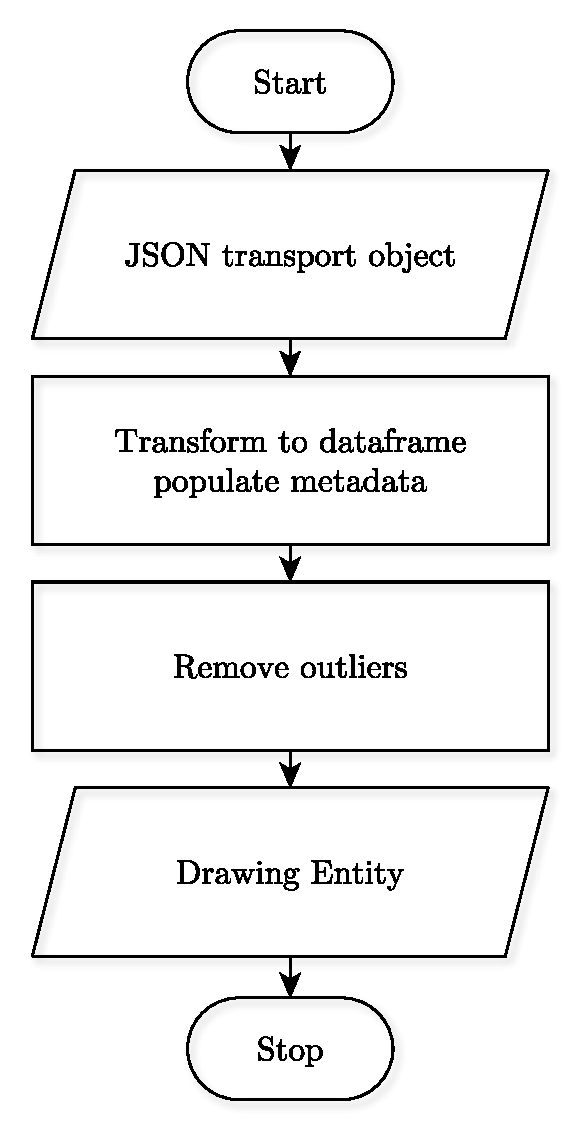
\includegraphics[width=0.30\textwidth]
    {images/data-preprocessing/flow-json-conversion-vertical}
    \caption{JSON to Drawing Entity Conversion --- Flow Diagram}
    \label{alg-drawing}
\end{figure}